\chapter{数学基础}

\section{位置与姿态的描述}

在进入 DH 参数法之前，我们必须先建立描述刚体位姿的数学工具。

\subsection{位置的描述}

三维空间中一个点的位置可以用一个 $3 \times 1$ 的列向量表示：

\begin{mydefinition}{位置向量}
	空间中点 $P$ 在坐标系 $\{A\}$ 中的位置记为
	\[
	{}^{A}\mathbf{p} = \begin{bmatrix} p_x \\ p_y \\ p_z \end{bmatrix} \in \R^3
	\]
	其中 $p_x, p_y, p_z$ 分别是点 $P$ 在坐标系 $\{A\}$ 三个坐标轴上的投影。
\end{mydefinition}

\subsection{姿态的描述——旋转矩阵}

刚体在空间中的姿态（朝向）需要一个参考坐标系。设坐标系 $\{B\}$ 固连于刚体上，其三个坐标轴的单位向量在参考系 $\{A\}$ 中表示为 $\hat{\mathbf{x}}_B, \hat{\mathbf{y}}_B, \hat{\mathbf{z}}_B$。将这些单位向量按列排成矩阵：

\begin{mydefinition}{旋转矩阵}
	坐标系 $\{B\}$ 相对于坐标系 $\{A\}$ 的旋转矩阵为
	\[
	{}^{A}_{B}\mathbf{R} = \begin{bmatrix}
		{}^{A}\hat{\mathbf{x}}_B & {}^{A}\hat{\mathbf{y}}_B & {}^{A}\hat{\mathbf{z}}_B
	\end{bmatrix} = \begin{bmatrix}
		r_{11} & r_{12} & r_{13} \\
		r_{21} & r_{22} & r_{23} \\
		r_{31} & r_{32} & r_{33}
	\end{bmatrix} \in \R^{3 \times 3}
	\]
\end{mydefinition}

旋转矩阵具有以下重要性质：

\begin{myTheorem}{旋转矩阵的性质}
	设 ${}^{A}_{B}\mathbf{R}$ 为旋转矩阵，则有：
	\begin{enumerate}
		\item \textbf{正交性}：${}^{A}_{B}\mathbf{R}\T \; {}^{A}_{B}\mathbf{R} = \mathbf{I}_3$
		\item \textbf{逆即为转置}：$({}^{A}_{B}\mathbf{R})^{-1} = ({}^{A}_{B}\mathbf{R})\T = {}^{B}_{A}\mathbf{R}$
		\item \textbf{行列式为1}：$\det({}^{A}_{B}\mathbf{R}) = 1$
		\item \textbf{群结构}：所有旋转矩阵构成特殊正交群 $\SO{3} = \{\mathbf{R} \in \R^{3\times 3} \mid \mathbf{R}\T\mathbf{R}=\mathbf{I},\;\det\mathbf{R}=1\}$
	\end{enumerate}
\end{myTheorem}

\subsection{绕坐标轴的基本旋转}

绕三个坐标轴旋转的矩阵是最基本的构件，任何旋转都可以分解为它们的有序组合。

\begin{figure}[htbp]
	\centering
	\begin{tikzpicture}[scale=1.2]
		% 绕Z轴
		\begin{scope}
			\draw[->] (0,0) -- (1.5,0) node[right] {$x$};
			\draw[->] (0,0) -- (0,1.5) node[above] {$y$};
			\draw[->, dashed] (0,0) -- (1.0,1.0) node[right] {$x'$};
			\draw[->, dashed] (0,0) -- (-1.0,1.0) node[left] {$y'$};
			\draw[->] (0,0) -- (0.3,0) arc (0:45:0.3);
			\node at (0.5,0.15) {$\theta$};
			\node at (0,-0.4) {绕 $z$ 轴旋转 $\theta$};
		\end{scope}
		
		\begin{scope}[xshift=4.5cm]
			\draw[->] (0,0) -- (1.5,0) node[right] {$y$};
			\draw[->] (0,0) -- (0,1.5) node[above] {$z$};
			\draw[->, dashed] (0,0) -- (1.0,1.0) node[right] {$y'$};
			\draw[->, dashed] (0,0) -- (-1.0,1.0) node[left] {$z'$};
			\node at (0,-0.4) {绕 $x$ 轴旋转 $\alpha$};
		\end{scope}
		
		\begin{scope}[xshift=9cm]
			\draw[->] (0,0) -- (1.5,0) node[right] {$z$};
			\draw[->] (0,0) -- (0,1.5) node[above] {$x$};
			\draw[->, dashed] (0,0) -- (1.0,1.0) node[right] {$z'$};
			\draw[->, dashed] (0,0) -- (-1.0,1.0) node[left] {$x'$};
			\node at (0,-0.4) {绕 $y$ 轴旋转 $\beta$};
		\end{scope}
	\end{tikzpicture}
	\caption{绕三个坐标轴的基本旋转}
\end{figure}

\[
\mathbf{R}_z(\theta) = \begin{bmatrix}
	\cos\theta & -\sin\theta & 0 \\
	\sin\theta &  \cos\theta & 0 \\
	0          &  0          & 1
\end{bmatrix}, \quad
\mathbf{R}_x(\alpha) = \begin{bmatrix}
	1 & 0         & 0          \\
	0 & \cos\alpha & -\sin\alpha \\
	0 & \sin\alpha &  \cos\alpha
\end{bmatrix}, \quad
\mathbf{R}_y(\beta) = \begin{bmatrix}
	 \cos\beta & 0 & \sin\beta \\
	 0         & 1 & 0         \\
	-\sin\beta & 0 & \cos\beta
\end{bmatrix}
\]

\section{齐次变换矩阵}

单独用旋转矩阵和平移向量只能分别描述姿态和位置。为将两者统一在一个框架中，我们引入\textbf{齐次变换矩阵}。

\begin{mydefinition}{齐次变换矩阵}
	坐标系 $\{B\}$ 相对于坐标系 $\{A\}$ 的齐次变换矩阵是一个 $4 \times 4$ 矩阵：
	\[
	{}^{A}_{B}\mathbf{T} = \begin{bmatrix}
		{}^{A}_{B}\mathbf{R} & {}^{A}\mathbf{p}_{B} \\
		\mathbf{0}_{1\times 3} & 1
	\end{bmatrix} = \begin{bmatrix}
		r_{11} & r_{12} & r_{13} & p_x \\
		r_{21} & r_{22} & r_{23} & p_y \\
		r_{31} & r_{32} & r_{33} & p_z \\
		0      & 0      & 0      & 1
	\end{bmatrix} \in \R^{4\times 4}
	\]
\end{mydefinition}

其中 ${}^{A}_{B}\mathbf{R} \in \SO{3}$ 为 $3\times3$ 旋转矩阵，${}^{A}\mathbf{p}_{B} \in \R^{3}$ 为坐标系 $\{B\}$ 原点在 $\{A\}$ 中的位置向量。

\begin{myTheorem}{齐次变换矩阵的性质}
	\begin{enumerate}
		\item \textbf{群结构}：所有齐次变换矩阵构成特殊欧氏群 $\SE{3}$。
		\item \textbf{逆变换}：
		\[
		{}^{A}_{B}\mathbf{T}^{-1} = {}^{B}_{A}\mathbf{T} = \begin{bmatrix}
			{}^{A}_{B}\mathbf{R}\T & -{}^{A}_{B}\mathbf{R}\T \; {}^{A}\mathbf{p}_{B} \\
			\mathbf{0} & 1
		\end{bmatrix}
		\]
		\item \textbf{复合变换}：级联变换只需矩阵相乘 ${}^{A}_{C}\mathbf{T} = {}^{A}_{B}\mathbf{T} \; {}^{B}_{C}\mathbf{T}$
	\end{enumerate}
\end{myTheorem}

\subsection{基本齐次变换}

平移变换和绕坐标轴的旋转变换是构成 DH 变换的基本单元：

\begin{myformula}
	\mathrm{Trans}(d_x, d_y, d_z) = \begin{bmatrix}
		1 & 0 & 0 & d_x \\
		0 & 1 & 0 & d_y \\
		0 & 0 & 1 & d_z \\
		0 & 0 & 0 & 1
	\end{bmatrix}
\end{myformula}

\begin{myformula}
	\mathrm{Rot}(z, \theta) = \begin{bmatrix}
		\cos\theta & -\sin\theta & 0 & 0 \\
		\sin\theta &  \cos\theta & 0 & 0 \\
		0          &  0          & 1 & 0 \\
		0          &  0          & 0 & 1
	\end{bmatrix}, \quad
	\mathrm{Rot}(x, \alpha) = \begin{bmatrix}
		1 & 0         & 0          & 0 \\
		0 & \cos\alpha & -\sin\alpha & 0 \\
		0 & \sin\alpha &  \cos\alpha & 0 \\
		0 & 0         & 0          & 1
	\end{bmatrix}
\end{myformula}

\subsection{齐次变换的几何意义}

齐次变换矩阵同时编码了旋转和平移两种操作。从坐标系变换角度看，${}^{A}_{B}\mathbf{T}$ 将坐标系 $\{B\}$ 中描述的向量变换到坐标系 $\{A\}$ 中：

\[
\begin{bmatrix} {}^{A}\mathbf{p} \\ 1 \end{bmatrix} = {}^{A}_{B}\mathbf{T} \begin{bmatrix} {}^{B}\mathbf{p} \\ 1 \end{bmatrix}
\]

\begin{figure}[htbp]
	\centering
	\begin{tikzpicture}[scale=1.3]
		% 坐标系A
		\draw[->, thick, blue] (0,0) -- (2,0) node[right] {$\hat{\mathbf{x}}_A$};
		\draw[->, thick, blue] (0,0) -- (0,2) node[above] {$\hat{\mathbf{y}}_A$};
		\filldraw (0,0) circle (1.5pt) node[below left] {$\{A\}$};
		
		% 坐标系B（旋转+平移）
		\begin{scope}[shift={(3,1.5)}, rotate=30]
			\draw[->, thick, red] (0,0) -- (1.5,0) node[right] {$\hat{\mathbf{x}}_B$};
			\draw[->, thick, red] (0,0) -- (0,1.5) node[above] {$\hat{\mathbf{y}}_B$};
			\filldraw (0,0) circle (1.5pt) node[below left] {$\{B\}$};
			
			% 点P
			\filldraw (1,0.8) circle (2pt) node[above right] {$P$};
			\draw[dashed] (0,0) -- (1,0.8);
		\end{scope}
		
		% 标注
		\draw[->, dashed, gray] (0,0) -- (3,1.5) node[midway, below] {${}^{A}\mathbf{p}_{B}$};
	\end{tikzpicture}
	\caption{坐标系变换：$\{B\}$ 相对于 $\{A\}$ 平移 $({}^{A}\mathbf{p}_{B})$ 并旋转}
\end{figure}

\section{坐标系的变换链}

对于 $n$ 个自由度的串联机器人，我们有 $n+1$ 个坐标系（包括基坐标系 $\{0\}$ 和工具坐标系 $\{n\}$）。从基座到末端的整体变换为各级变换的连乘：

\[
{}^{0}_{n}\mathbf{T} = {}^{0}_{1}\mathbf{T} \cdot {}^{1}_{2}\mathbf{T} \cdot {}^{2}_{3}\mathbf{T} \cdots {}^{n-1}_{n}\mathbf{T}
\]

\begin{figure}[htbp]
	\centering
	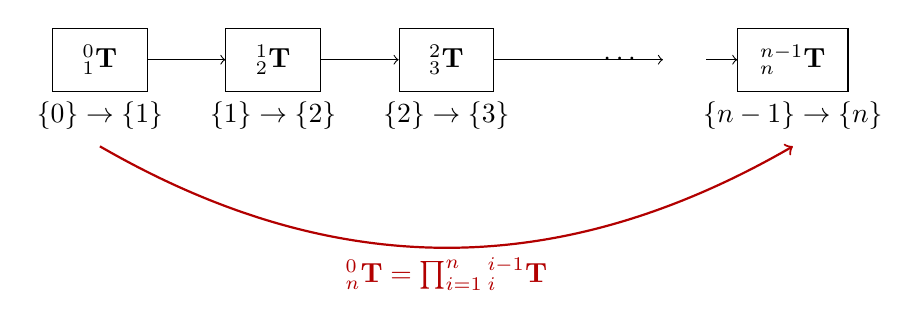
\begin{tikzpicture}[scale=1.1]
		% 变换链示意
		\node[draw, minimum width=1.2cm, minimum height=0.8cm] (T01) at (0,0) {${}^{0}_{1}\mathbf{T}$};
		\node[draw, minimum width=1.2cm, minimum height=0.8cm] (T12) at (2,0) {${}^{1}_{2}\mathbf{T}$};
		\node[draw, minimum width=1.2cm, minimum height=0.8cm] (T23) at (4,0) {${}^{2}_{3}\mathbf{T}$};
		\node at (6,0) {$\cdots$};
		\node[draw, minimum width=1.4cm, minimum height=0.8cm] (Tnn) at (8,0) {${}^{n-1}_{n}\mathbf{T}$};
		
		\draw[->] (T01) -- (T12);
		\draw[->] (T12) -- (T23);
		\draw[->] (T23) -- (6.5,0);
		\draw[->] (7,0) -- (Tnn);
		
		\node[below=0.3cm] at (0,-0.1) {$\{0\} \to \{1\}$};
		\node[below=0.3cm] at (2,-0.1) {$\{1\} \to \{2\}$};
		\node[below=0.3cm] at (4,-0.1) {$\{2\} \to \{3\}$};
		\node[below=0.3cm] at (8,-0.1) {$\{n-1\} \to \{n\}$};
		
		% 等效
		\draw[->, thick, red!70!black, bend right=30] (0,-1) to node[midway, below] {${}^{0}_{n}\mathbf{T} = \prod_{i=1}^{n} {}^{i-1}_{i}\mathbf{T}$} (8,-1);
	\end{tikzpicture}
	\caption{齐次变换的级联：各级变换矩阵依次相乘得到末端位姿}
\end{figure}

这正是正运动学的核心公式。DH 参数法的任务，就是将每一个 ${}^{i-1}_{i}\mathbf{T}$ 用最少且最系统的参数表达出来。
